% Options for packages loaded elsewhere
% Options for packages loaded elsewhere
\PassOptionsToPackage{unicode}{hyperref}
\PassOptionsToPackage{hyphens}{url}
%
\documentclass[
  english,
  russian,
  12pt,
  a4paper,
  DIV=11,
  numbers=noendperiod]{scrreprt}
\usepackage{xcolor}
\usepackage{amsmath,amssymb}
\setcounter{secnumdepth}{5}
\usepackage{iftex}
\ifPDFTeX
  \usepackage[T1]{fontenc}
  \usepackage[utf8]{inputenc}
  \usepackage{textcomp} % provide euro and other symbols
\else % if luatex or xetex
  \usepackage{unicode-math} % this also loads fontspec
  \defaultfontfeatures{Scale=MatchLowercase}
  \defaultfontfeatures[\rmfamily]{Ligatures=TeX,Scale=1}
\fi
\usepackage{lmodern}
\ifPDFTeX\else
  % xetex/luatex font selection
\fi
% Use upquote if available, for straight quotes in verbatim environments
\IfFileExists{upquote.sty}{\usepackage{upquote}}{}
\IfFileExists{microtype.sty}{% use microtype if available
  \usepackage[]{microtype}
  \UseMicrotypeSet[protrusion]{basicmath} % disable protrusion for tt fonts
}{}
\usepackage{setspace}
% Make \paragraph and \subparagraph free-standing
\makeatletter
\ifx\paragraph\undefined\else
  \let\oldparagraph\paragraph
  \renewcommand{\paragraph}{
    \@ifstar
      \xxxParagraphStar
      \xxxParagraphNoStar
  }
  \newcommand{\xxxParagraphStar}[1]{\oldparagraph*{#1}\mbox{}}
  \newcommand{\xxxParagraphNoStar}[1]{\oldparagraph{#1}\mbox{}}
\fi
\ifx\subparagraph\undefined\else
  \let\oldsubparagraph\subparagraph
  \renewcommand{\subparagraph}{
    \@ifstar
      \xxxSubParagraphStar
      \xxxSubParagraphNoStar
  }
  \newcommand{\xxxSubParagraphStar}[1]{\oldsubparagraph*{#1}\mbox{}}
  \newcommand{\xxxSubParagraphNoStar}[1]{\oldsubparagraph{#1}\mbox{}}
\fi
\makeatother

\usepackage{color}
\usepackage{fancyvrb}
\newcommand{\VerbBar}{|}
\newcommand{\VERB}{\Verb[commandchars=\\\{\}]}
\DefineVerbatimEnvironment{Highlighting}{Verbatim}{commandchars=\\\{\}}
% Add ',fontsize=\small' for more characters per line
\usepackage{framed}
\definecolor{shadecolor}{RGB}{241,243,245}
\newenvironment{Shaded}{\begin{snugshade}}{\end{snugshade}}
\newcommand{\AlertTok}[1]{\textcolor[rgb]{0.68,0.00,0.00}{#1}}
\newcommand{\AnnotationTok}[1]{\textcolor[rgb]{0.37,0.37,0.37}{#1}}
\newcommand{\AttributeTok}[1]{\textcolor[rgb]{0.40,0.45,0.13}{#1}}
\newcommand{\BaseNTok}[1]{\textcolor[rgb]{0.68,0.00,0.00}{#1}}
\newcommand{\BuiltInTok}[1]{\textcolor[rgb]{0.00,0.23,0.31}{#1}}
\newcommand{\CharTok}[1]{\textcolor[rgb]{0.13,0.47,0.30}{#1}}
\newcommand{\CommentTok}[1]{\textcolor[rgb]{0.37,0.37,0.37}{#1}}
\newcommand{\CommentVarTok}[1]{\textcolor[rgb]{0.37,0.37,0.37}{\textit{#1}}}
\newcommand{\ConstantTok}[1]{\textcolor[rgb]{0.56,0.35,0.01}{#1}}
\newcommand{\ControlFlowTok}[1]{\textcolor[rgb]{0.00,0.23,0.31}{\textbf{#1}}}
\newcommand{\DataTypeTok}[1]{\textcolor[rgb]{0.68,0.00,0.00}{#1}}
\newcommand{\DecValTok}[1]{\textcolor[rgb]{0.68,0.00,0.00}{#1}}
\newcommand{\DocumentationTok}[1]{\textcolor[rgb]{0.37,0.37,0.37}{\textit{#1}}}
\newcommand{\ErrorTok}[1]{\textcolor[rgb]{0.68,0.00,0.00}{#1}}
\newcommand{\ExtensionTok}[1]{\textcolor[rgb]{0.00,0.23,0.31}{#1}}
\newcommand{\FloatTok}[1]{\textcolor[rgb]{0.68,0.00,0.00}{#1}}
\newcommand{\FunctionTok}[1]{\textcolor[rgb]{0.28,0.35,0.67}{#1}}
\newcommand{\ImportTok}[1]{\textcolor[rgb]{0.00,0.46,0.62}{#1}}
\newcommand{\InformationTok}[1]{\textcolor[rgb]{0.37,0.37,0.37}{#1}}
\newcommand{\KeywordTok}[1]{\textcolor[rgb]{0.00,0.23,0.31}{\textbf{#1}}}
\newcommand{\NormalTok}[1]{\textcolor[rgb]{0.00,0.23,0.31}{#1}}
\newcommand{\OperatorTok}[1]{\textcolor[rgb]{0.37,0.37,0.37}{#1}}
\newcommand{\OtherTok}[1]{\textcolor[rgb]{0.00,0.23,0.31}{#1}}
\newcommand{\PreprocessorTok}[1]{\textcolor[rgb]{0.68,0.00,0.00}{#1}}
\newcommand{\RegionMarkerTok}[1]{\textcolor[rgb]{0.00,0.23,0.31}{#1}}
\newcommand{\SpecialCharTok}[1]{\textcolor[rgb]{0.37,0.37,0.37}{#1}}
\newcommand{\SpecialStringTok}[1]{\textcolor[rgb]{0.13,0.47,0.30}{#1}}
\newcommand{\StringTok}[1]{\textcolor[rgb]{0.13,0.47,0.30}{#1}}
\newcommand{\VariableTok}[1]{\textcolor[rgb]{0.07,0.07,0.07}{#1}}
\newcommand{\VerbatimStringTok}[1]{\textcolor[rgb]{0.13,0.47,0.30}{#1}}
\newcommand{\WarningTok}[1]{\textcolor[rgb]{0.37,0.37,0.37}{\textit{#1}}}

\usepackage{longtable,booktabs,array}
\usepackage{calc} % for calculating minipage widths
% Correct order of tables after \paragraph or \subparagraph
\usepackage{etoolbox}
\makeatletter
\patchcmd\longtable{\par}{\if@noskipsec\mbox{}\fi\par}{}{}
\makeatother
% Allow footnotes in longtable head/foot
\IfFileExists{footnotehyper.sty}{\usepackage{footnotehyper}}{\usepackage{footnote}}
\makesavenoteenv{longtable}
\usepackage{graphicx}
\makeatletter
\newsavebox\pandoc@box
\newcommand*\pandocbounded[1]{% scales image to fit in text height/width
  \sbox\pandoc@box{#1}%
  \Gscale@div\@tempa{\textheight}{\dimexpr\ht\pandoc@box+\dp\pandoc@box\relax}%
  \Gscale@div\@tempb{\linewidth}{\wd\pandoc@box}%
  \ifdim\@tempb\p@<\@tempa\p@\let\@tempa\@tempb\fi% select the smaller of both
  \ifdim\@tempa\p@<\p@\scalebox{\@tempa}{\usebox\pandoc@box}%
  \else\usebox{\pandoc@box}%
  \fi%
}
% Set default figure placement to htbp
\def\fps@figure{htbp}
\makeatother



\ifLuaTeX
\usepackage[bidi=basic,provide=*]{babel}
\else
\usepackage[bidi=default,provide=*]{babel}
\fi
% get rid of language-specific shorthands (see #6817):
\let\LanguageShortHands\languageshorthands
\def\languageshorthands#1{}


\setlength{\emergencystretch}{3em} % prevent overfull lines

\providecommand{\tightlist}{%
  \setlength{\itemsep}{0pt}\setlength{\parskip}{0pt}}



 
\usepackage[style=gost-numeric,backend=biber,langhook=extras,autolang=other*]{biblatex}
\addbibresource{bib/cite.bib}

\usepackage[]{csquotes}

\usepackage{indentfirst}
\usepackage{float}
\floatplacement{figure}{H}
\IfFileExists{plex-otf.sty}{
  %% Full TeXlive
  \usepackage[
    % math,
    RM={Scale=0.94},SS={Scale=0.94},SScon={Scale=0.94},TT={Scale=MatchLowercase,FakeStretch=0.9},
    DefaultFeatures={Ligatures=Common}
  ]{plex-otf}
  % \usepackage[Scale=MatchUppercase]{juliamono}
}{
  %% TinyTeX
  \usepackage{libertine}
}
\KOMAoption{captions}{tableheading}
\makeatletter
\@ifpackageloaded{caption}{}{\usepackage{caption}}
\AtBeginDocument{%
\ifdefined\contentsname
  \renewcommand*\contentsname{Содержание}
\else
  \newcommand\contentsname{Содержание}
\fi
\ifdefined\listfigurename
  \renewcommand*\listfigurename{Список иллюстраций}
\else
  \newcommand\listfigurename{Список иллюстраций}
\fi
\ifdefined\listtablename
  \renewcommand*\listtablename{Список таблиц}
\else
  \newcommand\listtablename{Список таблиц}
\fi
\ifdefined\figurename
  \renewcommand*\figurename{Рисунок}
\else
  \newcommand\figurename{Рисунок}
\fi
\ifdefined\tablename
  \renewcommand*\tablename{Таблица}
\else
  \newcommand\tablename{Таблица}
\fi
}
\@ifpackageloaded{float}{}{\usepackage{float}}
\floatstyle{ruled}
\@ifundefined{c@chapter}{\newfloat{codelisting}{h}{lop}}{\newfloat{codelisting}{h}{lop}[chapter]}
\floatname{codelisting}{Список}
\newcommand*\listoflistings{\listof{codelisting}{Листинги}}
\makeatother
\makeatletter
\makeatother
\makeatletter
\@ifpackageloaded{caption}{}{\usepackage{caption}}
\@ifpackageloaded{subcaption}{}{\usepackage{subcaption}}
\makeatother
\usepackage{bookmark}
\IfFileExists{xurl.sty}{\usepackage{xurl}}{} % add URL line breaks if available
\urlstyle{same}
\hypersetup{
  pdftitle={Лабораторная работа №3: Daisyworld},
  pdfauthor={Федорова Анжелика Игоревна},
  pdflang={ru-RU},
  hidelinks,
  pdfcreator={LaTeX via pandoc}}


\title{Лабораторная работа №3: Daisyworld}
\author{Федорова Анжелика Игоревна}
\date{}
\begin{document}
\maketitle

\renewcommand*\contentsname{Содержание}
{
\setcounter{tocdepth}{1}
\tableofcontents
}
\listoffigures
\listoftables

\setstretch{1.5}
\chapter{Цель
работы}\label{ux446ux435ux43bux44c-ux440ux430ux431ux43eux442ux44b}

Реализовать агентную модель Daisyworld, провести вычислительные
эксперименты и исследовать поведение системы при различных параметрах.

\chapter{Задание}\label{ux437ux430ux434ux430ux43dux438ux435}

В ходе работы необходимо:

\begin{enumerate}
\def\labelenumi{\arabic{enumi}.}
\tightlist
\item
  Создать структуру проекта
\item
  Установить необходимые пакеты
\item
  Реализовать модель Daisyworld
\item
  Выполнить визуализацию
\item
  Построить графики динамики
\item
  Провести параметрические эксперименты
\item
  Оформить отчёт
\end{enumerate}

\chapter{Ход
работы}\label{ux445ux43eux434-ux440ux430ux431ux43eux442ux44b}

\section{1. Подготовка
проекта}\label{ux43fux43eux434ux433ux43eux442ux43eux432ux43aux430-ux43fux440ux43eux435ux43aux442ux430}

Была создана структура проекта с использованием \texttt{DrWatson}:

\begin{itemize}
\tightlist
\item
  \texttt{src/} --- код модели
\item
  \texttt{scripts/} --- исполняемые скрипты
\item
  \texttt{plots/} --- результаты
\end{itemize}

Установлены пакеты:

\begin{Shaded}
\begin{Highlighting}[]
\ImportTok{using} \BuiltInTok{Pkg}
\BuiltInTok{Pkg}\NormalTok{.}\FunctionTok{add}\NormalTok{([}\StringTok{"Agents"}\NormalTok{, }\StringTok{"CairoMakie"}\NormalTok{, }\StringTok{"DataFrames"}\NormalTok{, }\StringTok{"StatsBase"}\NormalTok{, }\StringTok{"Plots"}\NormalTok{, }\StringTok{"DrWatson"}\NormalTok{])}
\end{Highlighting}
\end{Shaded}

\section{2. Реализация
модели}\label{ux440ux435ux430ux43bux438ux437ux430ux446ux438ux44f-ux43cux43eux434ux435ux43bux438}

Модель реализована в файле:

\begin{Shaded}
\begin{Highlighting}[]
\ImportTok{using} \BuiltInTok{Agents}
\ImportTok{import} \BuiltInTok{StatsBase}
\ImportTok{using} \BuiltInTok{Random}

\PreprocessorTok{@agent} \KeywordTok{struct} \FunctionTok{Daisy}\NormalTok{(GridAgent\{}\FloatTok{2}\NormalTok{\})}
\NormalTok{    breed}\OperatorTok{::}\DataTypeTok{Symbol}
\NormalTok{    age}\OperatorTok{::}\DataTypeTok{Int}
\NormalTok{    albedo}\OperatorTok{::}\DataTypeTok{Float64 }\CommentTok{\# 0{-}1 fraction}
\KeywordTok{end}

\KeywordTok{function} \FunctionTok{update\_surface\_temperature!}\NormalTok{(pos, model)}
\NormalTok{    absorbed\_luminosity }\OperatorTok{=} \ControlFlowTok{if} \FunctionTok{isempty}\NormalTok{(pos, model) }\CommentTok{\# no daisy}
\NormalTok{        (}\FloatTok{1} \OperatorTok{{-}}\NormalTok{ model.surface\_albedo) }\OperatorTok{*}\NormalTok{ model.solar\_luminosity}
    \ControlFlowTok{else}
\NormalTok{        daisy }\OperatorTok{=}\NormalTok{ model[}\FunctionTok{id\_in\_position}\NormalTok{(pos, model)]}
\NormalTok{        (}\FloatTok{1} \OperatorTok{{-}}\NormalTok{ daisy.albedo) }\OperatorTok{*}\NormalTok{ model.solar\_luminosity}
    \ControlFlowTok{end}
\NormalTok{    local\_heating }\OperatorTok{=}\NormalTok{ absorbed\_luminosity }\OperatorTok{\textgreater{}} \FloatTok{0}\NormalTok{ ? }\FloatTok{72} \OperatorTok{*} \FunctionTok{log}\NormalTok{(absorbed\_luminosity) }\OperatorTok{+} \FloatTok{80} \OperatorTok{:} \FloatTok{80}
\NormalTok{    model.temperature[pos}\OperatorTok{...}\NormalTok{] }\OperatorTok{=}\NormalTok{ (model.temperature[pos}\OperatorTok{...}\NormalTok{] }\OperatorTok{+}\NormalTok{ local\_heating) }\OperatorTok{/} \FloatTok{2}
\KeywordTok{end}

\KeywordTok{function} \FunctionTok{diffuse\_temperature!}\NormalTok{(pos, model)}
\NormalTok{    ratio }\OperatorTok{=}\NormalTok{ model.ratio }\CommentTok{\# diffusion ratio}
\NormalTok{    npos }\OperatorTok{=} \FunctionTok{nearby\_positions}\NormalTok{(pos, model)}
\NormalTok{    model.temperature[pos}\OperatorTok{...}\NormalTok{] }\OperatorTok{=}
\NormalTok{        (}\FloatTok{1} \OperatorTok{{-}}\NormalTok{ ratio) }\OperatorTok{*}\NormalTok{ model.temperature[pos}\OperatorTok{...}\NormalTok{] }\OperatorTok{+}
        \FunctionTok{sum}\NormalTok{(model.temperature[p}\OperatorTok{...}\NormalTok{] }\ControlFlowTok{for}\NormalTok{ p }\KeywordTok{in}\NormalTok{ npos) }\OperatorTok{*} \FloatTok{0.125} \OperatorTok{*}\NormalTok{ ratio}
\ControlFlowTok{end}

\KeywordTok{function} \FunctionTok{propagate!}\NormalTok{(pos, model)}
    \FunctionTok{isempty}\NormalTok{(pos, model) }\OperatorTok{\&\&} \ControlFlowTok{return}
\NormalTok{    daisy }\OperatorTok{=}\NormalTok{ model[}\FunctionTok{id\_in\_position}\NormalTok{(pos, model)]}
\NormalTok{    temperature }\OperatorTok{=}\NormalTok{ model.temperature[pos}\OperatorTok{...}\NormalTok{]}
\NormalTok{    seed\_threshold }\OperatorTok{=}\NormalTok{ (}\FloatTok{0.1457} \OperatorTok{*}\NormalTok{ temperature }\OperatorTok{{-}} \FloatTok{0.0032} \OperatorTok{*}\NormalTok{ temperature}\OperatorTok{\^{}}\FloatTok{2}\NormalTok{) }\OperatorTok{{-}} \FloatTok{0.6443}
    \ControlFlowTok{if} \FunctionTok{rand}\NormalTok{(}\FunctionTok{abmrng}\NormalTok{(model)) }\OperatorTok{\textless{}}\NormalTok{ seed\_threshold}
\NormalTok{        empty\_near\_pos }\OperatorTok{=} \FunctionTok{random\_nearby\_position}\NormalTok{(pos, model, }\FloatTok{1}\NormalTok{, npos }\OperatorTok{{-}\textgreater{}} \FunctionTok{isempty}\NormalTok{(npos, model))}
        \ControlFlowTok{if}\NormalTok{ !}\FunctionTok{isnothing}\NormalTok{(empty\_near\_pos)}
            \FunctionTok{add\_agent!}\NormalTok{(empty\_near\_pos, model, daisy.breed, }\FloatTok{0}\NormalTok{, daisy.albedo)}
        \ControlFlowTok{end}
    \ControlFlowTok{end}
\KeywordTok{end}

\KeywordTok{function} \FunctionTok{daisy\_step!}\NormalTok{(agent}\OperatorTok{::}\DataTypeTok{Daisy}\NormalTok{, model)}
\NormalTok{    agent.age }\OperatorTok{+=} \FloatTok{1}
\NormalTok{    agent.age }\OperatorTok{≥}\NormalTok{ model.max\_age }\OperatorTok{\&\&} \FunctionTok{remove\_agent!}\NormalTok{(agent, model)}
\KeywordTok{end}

\KeywordTok{function} \FunctionTok{daisyworld\_step!}\NormalTok{(model)}
    \ControlFlowTok{for}\NormalTok{ p }\KeywordTok{in} \FunctionTok{positions}\NormalTok{(model)}
        \FunctionTok{update\_surface\_temperature!}\NormalTok{(p, model)}
        \FunctionTok{diffuse\_temperature!}\NormalTok{(p, model)}
        \FunctionTok{propagate!}\NormalTok{(p, model)}
    \ControlFlowTok{end}
\NormalTok{    model.tick }\OperatorTok{=}\NormalTok{ model.tick }\OperatorTok{+} \FloatTok{1}
    \FunctionTok{solar\_activity!}\NormalTok{(model)}
\KeywordTok{end}

\KeywordTok{function} \FunctionTok{solar\_activity!}\NormalTok{(model)}
    \ControlFlowTok{if}\NormalTok{ model.scenario }\OperatorTok{==} \OperatorTok{:}\NormalTok{ramp}
        \ControlFlowTok{if}\NormalTok{ model.tick }\OperatorTok{\textgreater{}} \FloatTok{200} \OperatorTok{\&\&}\NormalTok{ model.tick }\OperatorTok{≤} \FloatTok{400}
\NormalTok{            model.solar\_luminosity }\OperatorTok{+=}\NormalTok{ model.solar\_change}
        \ControlFlowTok{end}
        \ControlFlowTok{if}\NormalTok{ model.tick }\OperatorTok{\textgreater{}} \FloatTok{500} \OperatorTok{\&\&}\NormalTok{ model.tick }\OperatorTok{≤} \FloatTok{750}
\NormalTok{            model.solar\_luminosity }\OperatorTok{{-}=}\NormalTok{ model.solar\_change }\OperatorTok{/} \FloatTok{2}
        \ControlFlowTok{end}
    \ControlFlowTok{elseif}\NormalTok{ model.scenario }\OperatorTok{==} \OperatorTok{:}\NormalTok{change}
\NormalTok{        model.solar\_luminosity }\OperatorTok{+=}\NormalTok{ model.solar\_change}
    \ControlFlowTok{end}
\KeywordTok{end}

\ImportTok{using} \BuiltInTok{Random}

\KeywordTok{function} \FunctionTok{daisyworld}\NormalTok{(;}
\NormalTok{    griddims }\OperatorTok{=}\NormalTok{ (}\FloatTok{30}\NormalTok{, }\FloatTok{30}\NormalTok{),}
\NormalTok{    max\_age }\OperatorTok{=} \FloatTok{25}\NormalTok{,}
\NormalTok{    init\_white }\OperatorTok{=} \FloatTok{0.2}\NormalTok{, }\CommentTok{\# \% cover of the world surface of white breed}
\NormalTok{    init\_black }\OperatorTok{=} \FloatTok{0.2}\NormalTok{, }\CommentTok{\# \% cover of the world surface of black breed}
\NormalTok{    albedo\_white }\OperatorTok{=} \FloatTok{0.75}\NormalTok{,}
\NormalTok{    albedo\_black }\OperatorTok{=} \FloatTok{0.25}\NormalTok{,}
\NormalTok{    surface\_albedo }\OperatorTok{=} \FloatTok{0.4}\NormalTok{,}
\NormalTok{    solar\_change }\OperatorTok{=} \FloatTok{0.005}\NormalTok{,}
\NormalTok{    solar\_luminosity }\OperatorTok{=} \FloatTok{1.0}\NormalTok{, }\CommentTok{\# initial luminosity}
\NormalTok{    scenario }\OperatorTok{=} \OperatorTok{:}\NormalTok{default,}
\NormalTok{    seed }\OperatorTok{=} \FloatTok{165}\NormalTok{,}
\NormalTok{)}

\NormalTok{    rng }\OperatorTok{=} \FunctionTok{MersenneTwister}\NormalTok{(seed)}
\NormalTok{    space }\OperatorTok{=} \FunctionTok{GridSpaceSingle}\NormalTok{(griddims)}
\NormalTok{    properties }\OperatorTok{=}\NormalTok{ (;max\_age, surface\_albedo, solar\_luminosity, solar\_change, scenario,}
\NormalTok{        tick }\OperatorTok{=} \FloatTok{0}\NormalTok{, ratio }\OperatorTok{=} \FloatTok{0.5}\NormalTok{, temperature }\OperatorTok{=} \FunctionTok{zeros}\NormalTok{(griddims)}
\NormalTok{    )}
\NormalTok{    properties }\OperatorTok{=} \FunctionTok{Dict}\NormalTok{(k}\OperatorTok{=\textgreater{}}\NormalTok{v }\ControlFlowTok{for}\NormalTok{ (k,v) }\KeywordTok{in} \FunctionTok{pairs}\NormalTok{(properties))}

\NormalTok{    model }\OperatorTok{=} \FunctionTok{StandardABM}\NormalTok{(Daisy, space; properties, rng, agent\_step! }\OperatorTok{=}\NormalTok{ daisy\_step!, model\_step! }\OperatorTok{=}\NormalTok{ daisyworld\_step!)}

\NormalTok{    grid }\OperatorTok{=} \FunctionTok{collect}\NormalTok{(}\FunctionTok{positions}\NormalTok{(model))}
\NormalTok{    num\_positions }\OperatorTok{=} \FunctionTok{prod}\NormalTok{(griddims)}
\NormalTok{    white\_positions }\OperatorTok{=}
\NormalTok{        StatsBase.}\FunctionTok{sample}\NormalTok{(grid, }\FunctionTok{Int}\NormalTok{(init\_white }\OperatorTok{*}\NormalTok{ num\_positions); replace }\OperatorTok{=} \ConstantTok{false}\NormalTok{)}
    \ControlFlowTok{for}\NormalTok{ wp }\KeywordTok{in}\NormalTok{ white\_positions}
        \FunctionTok{add\_agent!}\NormalTok{(wp, Daisy, model, }\OperatorTok{:}\NormalTok{white, }\FunctionTok{rand}\NormalTok{(}\FunctionTok{abmrng}\NormalTok{(model), }\FloatTok{0}\OperatorTok{:}\NormalTok{max\_age), albedo\_white)}
    \ControlFlowTok{end}
\NormalTok{    allowed }\OperatorTok{=} \FunctionTok{setdiff}\NormalTok{(grid, white\_positions)}
\NormalTok{    black\_positions }\OperatorTok{=}
\NormalTok{        StatsBase.}\FunctionTok{sample}\NormalTok{(allowed, }\FunctionTok{Int}\NormalTok{(init\_black }\OperatorTok{*}\NormalTok{ num\_positions); replace }\OperatorTok{=} \ConstantTok{false}\NormalTok{)}
    \ControlFlowTok{for}\NormalTok{ bp }\KeywordTok{in}\NormalTok{ black\_positions}
        \FunctionTok{add\_agent!}\NormalTok{(bp, Daisy, model, }\OperatorTok{:}\NormalTok{black, }\FunctionTok{rand}\NormalTok{(}\FunctionTok{abmrng}\NormalTok{(model), }\FloatTok{0}\OperatorTok{:}\NormalTok{max\_age), albedo\_black)}
    \ControlFlowTok{end}

    \ControlFlowTok{for}\NormalTok{ p }\KeywordTok{in} \FunctionTok{positions}\NormalTok{(model)}
        \FunctionTok{update\_surface\_temperature!}\NormalTok{(p, model)}
    \ControlFlowTok{end}

    \ControlFlowTok{return}\NormalTok{ model}
\ControlFlowTok{end}
\end{Highlighting}
\end{Shaded}

Описание:

\begin{itemize}
\item
  агенты: маргаритки (чёрные и белые)
\item
  среда: сетка 30×30
\item
  реализованы процессы:

  \begin{itemize}
  \tightlist
  \item
    нагрев поверхности
  \item
    диффузия температуры
  \item
    размножение
  \item
    старение
  \end{itemize}
\end{itemize}

Подключение модели:

\begin{Shaded}
\begin{Highlighting}[]
\ImportTok{using} \BuiltInTok{Agents}
\ImportTok{import} \BuiltInTok{StatsBase}
\ImportTok{using} \BuiltInTok{Random}

\PreprocessorTok{@agent} \KeywordTok{struct} \FunctionTok{Daisy}\NormalTok{(GridAgent\{}\FloatTok{2}\NormalTok{\})}
\NormalTok{    breed}\OperatorTok{::}\DataTypeTok{Symbol}
\NormalTok{    age}\OperatorTok{::}\DataTypeTok{Int}
\NormalTok{    albedo}\OperatorTok{::}\DataTypeTok{Float64 }\CommentTok{\# 0{-}1 fraction}
\KeywordTok{end}

\KeywordTok{function} \FunctionTok{update\_surface\_temperature!}\NormalTok{(pos, model)}
\NormalTok{    absorbed\_luminosity }\OperatorTok{=} \ControlFlowTok{if} \FunctionTok{isempty}\NormalTok{(pos, model) }\CommentTok{\# no daisy}
\NormalTok{        (}\FloatTok{1} \OperatorTok{{-}}\NormalTok{ model.surface\_albedo) }\OperatorTok{*}\NormalTok{ model.solar\_luminosity}
    \ControlFlowTok{else}
\NormalTok{        daisy }\OperatorTok{=}\NormalTok{ model[}\FunctionTok{id\_in\_position}\NormalTok{(pos, model)]}
\NormalTok{        (}\FloatTok{1} \OperatorTok{{-}}\NormalTok{ daisy.albedo) }\OperatorTok{*}\NormalTok{ model.solar\_luminosity}
    \ControlFlowTok{end}
\NormalTok{    local\_heating }\OperatorTok{=}\NormalTok{ absorbed\_luminosity }\OperatorTok{\textgreater{}} \FloatTok{0}\NormalTok{ ? }\FloatTok{72} \OperatorTok{*} \FunctionTok{log}\NormalTok{(absorbed\_luminosity) }\OperatorTok{+} \FloatTok{80} \OperatorTok{:} \FloatTok{80}
\NormalTok{    model.temperature[pos}\OperatorTok{...}\NormalTok{] }\OperatorTok{=}\NormalTok{ (model.temperature[pos}\OperatorTok{...}\NormalTok{] }\OperatorTok{+}\NormalTok{ local\_heating) }\OperatorTok{/} \FloatTok{2}
\KeywordTok{end}

\KeywordTok{function} \FunctionTok{diffuse\_temperature!}\NormalTok{(pos, model)}
\NormalTok{    ratio }\OperatorTok{=}\NormalTok{ model.ratio }\CommentTok{\# diffusion ratio}
\NormalTok{    npos }\OperatorTok{=} \FunctionTok{nearby\_positions}\NormalTok{(pos, model)}
\NormalTok{    model.temperature[pos}\OperatorTok{...}\NormalTok{] }\OperatorTok{=}
\NormalTok{        (}\FloatTok{1} \OperatorTok{{-}}\NormalTok{ ratio) }\OperatorTok{*}\NormalTok{ model.temperature[pos}\OperatorTok{...}\NormalTok{] }\OperatorTok{+}
        \FunctionTok{sum}\NormalTok{(model.temperature[p}\OperatorTok{...}\NormalTok{] }\ControlFlowTok{for}\NormalTok{ p }\KeywordTok{in}\NormalTok{ npos) }\OperatorTok{*} \FloatTok{0.125} \OperatorTok{*}\NormalTok{ ratio}
\ControlFlowTok{end}

\KeywordTok{function} \FunctionTok{propagate!}\NormalTok{(pos, model)}
    \FunctionTok{isempty}\NormalTok{(pos, model) }\OperatorTok{\&\&} \ControlFlowTok{return}
\NormalTok{    daisy }\OperatorTok{=}\NormalTok{ model[}\FunctionTok{id\_in\_position}\NormalTok{(pos, model)]}
\NormalTok{    temperature }\OperatorTok{=}\NormalTok{ model.temperature[pos}\OperatorTok{...}\NormalTok{]}
\NormalTok{    seed\_threshold }\OperatorTok{=}\NormalTok{ (}\FloatTok{0.1457} \OperatorTok{*}\NormalTok{ temperature }\OperatorTok{{-}} \FloatTok{0.0032} \OperatorTok{*}\NormalTok{ temperature}\OperatorTok{\^{}}\FloatTok{2}\NormalTok{) }\OperatorTok{{-}} \FloatTok{0.6443}
    \ControlFlowTok{if} \FunctionTok{rand}\NormalTok{(}\FunctionTok{abmrng}\NormalTok{(model)) }\OperatorTok{\textless{}}\NormalTok{ seed\_threshold}
\NormalTok{        empty\_near\_pos }\OperatorTok{=} \FunctionTok{random\_nearby\_position}\NormalTok{(pos, model, }\FloatTok{1}\NormalTok{, npos }\OperatorTok{{-}\textgreater{}} \FunctionTok{isempty}\NormalTok{(npos, model))}
        \ControlFlowTok{if}\NormalTok{ !}\FunctionTok{isnothing}\NormalTok{(empty\_near\_pos)}
            \FunctionTok{add\_agent!}\NormalTok{(empty\_near\_pos, model, daisy.breed, }\FloatTok{0}\NormalTok{, daisy.albedo)}
        \ControlFlowTok{end}
    \ControlFlowTok{end}
\KeywordTok{end}

\KeywordTok{function} \FunctionTok{daisy\_step!}\NormalTok{(agent}\OperatorTok{::}\DataTypeTok{Daisy}\NormalTok{, model)}
\NormalTok{    agent.age }\OperatorTok{+=} \FloatTok{1}
\NormalTok{    agent.age }\OperatorTok{≥}\NormalTok{ model.max\_age }\OperatorTok{\&\&} \FunctionTok{remove\_agent!}\NormalTok{(agent, model)}
\KeywordTok{end}

\KeywordTok{function} \FunctionTok{daisyworld\_step!}\NormalTok{(model)}
    \ControlFlowTok{for}\NormalTok{ p }\KeywordTok{in} \FunctionTok{positions}\NormalTok{(model)}
        \FunctionTok{update\_surface\_temperature!}\NormalTok{(p, model)}
        \FunctionTok{diffuse\_temperature!}\NormalTok{(p, model)}
        \FunctionTok{propagate!}\NormalTok{(p, model)}
    \ControlFlowTok{end}
\NormalTok{    model.tick }\OperatorTok{=}\NormalTok{ model.tick }\OperatorTok{+} \FloatTok{1}
    \FunctionTok{solar\_activity!}\NormalTok{(model)}
\KeywordTok{end}

\KeywordTok{function} \FunctionTok{solar\_activity!}\NormalTok{(model)}
    \ControlFlowTok{if}\NormalTok{ model.scenario }\OperatorTok{==} \OperatorTok{:}\NormalTok{ramp}
        \ControlFlowTok{if}\NormalTok{ model.tick }\OperatorTok{\textgreater{}} \FloatTok{200} \OperatorTok{\&\&}\NormalTok{ model.tick }\OperatorTok{≤} \FloatTok{400}
\NormalTok{            model.solar\_luminosity }\OperatorTok{+=}\NormalTok{ model.solar\_change}
        \ControlFlowTok{end}
        \ControlFlowTok{if}\NormalTok{ model.tick }\OperatorTok{\textgreater{}} \FloatTok{500} \OperatorTok{\&\&}\NormalTok{ model.tick }\OperatorTok{≤} \FloatTok{750}
\NormalTok{            model.solar\_luminosity }\OperatorTok{{-}=}\NormalTok{ model.solar\_change }\OperatorTok{/} \FloatTok{2}
        \ControlFlowTok{end}
    \ControlFlowTok{elseif}\NormalTok{ model.scenario }\OperatorTok{==} \OperatorTok{:}\NormalTok{change}
\NormalTok{        model.solar\_luminosity }\OperatorTok{+=}\NormalTok{ model.solar\_change}
    \ControlFlowTok{end}
\KeywordTok{end}

\ImportTok{using} \BuiltInTok{Random}

\KeywordTok{function} \FunctionTok{daisyworld}\NormalTok{(;}
\NormalTok{    griddims }\OperatorTok{=}\NormalTok{ (}\FloatTok{30}\NormalTok{, }\FloatTok{30}\NormalTok{),}
\NormalTok{    max\_age }\OperatorTok{=} \FloatTok{25}\NormalTok{,}
\NormalTok{    init\_white }\OperatorTok{=} \FloatTok{0.2}\NormalTok{, }\CommentTok{\# \% cover of the world surface of white breed}
\NormalTok{    init\_black }\OperatorTok{=} \FloatTok{0.2}\NormalTok{, }\CommentTok{\# \% cover of the world surface of black breed}
\NormalTok{    albedo\_white }\OperatorTok{=} \FloatTok{0.75}\NormalTok{,}
\NormalTok{    albedo\_black }\OperatorTok{=} \FloatTok{0.25}\NormalTok{,}
\NormalTok{    surface\_albedo }\OperatorTok{=} \FloatTok{0.4}\NormalTok{,}
\NormalTok{    solar\_change }\OperatorTok{=} \FloatTok{0.005}\NormalTok{,}
\NormalTok{    solar\_luminosity }\OperatorTok{=} \FloatTok{1.0}\NormalTok{, }\CommentTok{\# initial luminosity}
\NormalTok{    scenario }\OperatorTok{=} \OperatorTok{:}\NormalTok{default,}
\NormalTok{    seed }\OperatorTok{=} \FloatTok{165}\NormalTok{,}
\NormalTok{)}

\NormalTok{    rng }\OperatorTok{=} \FunctionTok{MersenneTwister}\NormalTok{(seed)}
\NormalTok{    space }\OperatorTok{=} \FunctionTok{GridSpaceSingle}\NormalTok{(griddims)}
\NormalTok{    properties }\OperatorTok{=}\NormalTok{ (;max\_age, surface\_albedo, solar\_luminosity, solar\_change, scenario,}
\NormalTok{        tick }\OperatorTok{=} \FloatTok{0}\NormalTok{, ratio }\OperatorTok{=} \FloatTok{0.5}\NormalTok{, temperature }\OperatorTok{=} \FunctionTok{zeros}\NormalTok{(griddims)}
\NormalTok{    )}
\NormalTok{    properties }\OperatorTok{=} \FunctionTok{Dict}\NormalTok{(k}\OperatorTok{=\textgreater{}}\NormalTok{v }\ControlFlowTok{for}\NormalTok{ (k,v) }\KeywordTok{in} \FunctionTok{pairs}\NormalTok{(properties))}

\NormalTok{    model }\OperatorTok{=} \FunctionTok{StandardABM}\NormalTok{(Daisy, space; properties, rng, agent\_step! }\OperatorTok{=}\NormalTok{ daisy\_step!, model\_step! }\OperatorTok{=}\NormalTok{ daisyworld\_step!)}

\NormalTok{    grid }\OperatorTok{=} \FunctionTok{collect}\NormalTok{(}\FunctionTok{positions}\NormalTok{(model))}
\NormalTok{    num\_positions }\OperatorTok{=} \FunctionTok{prod}\NormalTok{(griddims)}
\NormalTok{    white\_positions }\OperatorTok{=}
\NormalTok{        StatsBase.}\FunctionTok{sample}\NormalTok{(grid, }\FunctionTok{Int}\NormalTok{(init\_white }\OperatorTok{*}\NormalTok{ num\_positions); replace }\OperatorTok{=} \ConstantTok{false}\NormalTok{)}
    \ControlFlowTok{for}\NormalTok{ wp }\KeywordTok{in}\NormalTok{ white\_positions}
        \FunctionTok{add\_agent!}\NormalTok{(wp, Daisy, model, }\OperatorTok{:}\NormalTok{white, }\FunctionTok{rand}\NormalTok{(}\FunctionTok{abmrng}\NormalTok{(model), }\FloatTok{0}\OperatorTok{:}\NormalTok{max\_age), albedo\_white)}
    \ControlFlowTok{end}
\NormalTok{    allowed }\OperatorTok{=} \FunctionTok{setdiff}\NormalTok{(grid, white\_positions)}
\NormalTok{    black\_positions }\OperatorTok{=}
\NormalTok{        StatsBase.}\FunctionTok{sample}\NormalTok{(allowed, }\FunctionTok{Int}\NormalTok{(init\_black }\OperatorTok{*}\NormalTok{ num\_positions); replace }\OperatorTok{=} \ConstantTok{false}\NormalTok{)}
    \ControlFlowTok{for}\NormalTok{ bp }\KeywordTok{in}\NormalTok{ black\_positions}
        \FunctionTok{add\_agent!}\NormalTok{(bp, Daisy, model, }\OperatorTok{:}\NormalTok{black, }\FunctionTok{rand}\NormalTok{(}\FunctionTok{abmrng}\NormalTok{(model), }\FloatTok{0}\OperatorTok{:}\NormalTok{max\_age), albedo\_black)}
    \ControlFlowTok{end}

    \ControlFlowTok{for}\NormalTok{ p }\KeywordTok{in} \FunctionTok{positions}\NormalTok{(model)}
        \FunctionTok{update\_surface\_temperature!}\NormalTok{(p, model)}
    \ControlFlowTok{end}

    \ControlFlowTok{return}\NormalTok{ model}
\ControlFlowTok{end}
\end{Highlighting}
\end{Shaded}

\section{3. Базовая
визуализация}\label{ux431ux430ux437ux43eux432ux430ux44f-ux432ux438ux437ux443ux430ux43bux438ux437ux430ux446ux438ux44f}

Скрипт:

\begin{Shaded}
\begin{Highlighting}[]
\ImportTok{using} \BuiltInTok{DrWatson}
\PreprocessorTok{@quickactivate} \StringTok{"project"}
\ImportTok{using} \BuiltInTok{Agents}
\ImportTok{using} \BuiltInTok{DataFrames}
\ImportTok{using} \BuiltInTok{Plots}


\FunctionTok{include}\NormalTok{(}\FunctionTok{srcdir}\NormalTok{(}\StringTok{"daisyworld.jl"}\NormalTok{))}

\ImportTok{using} \BuiltInTok{CairoMakie}
\NormalTok{model }\OperatorTok{=} \FunctionTok{daisyworld}\NormalTok{()}

\FunctionTok{daisycolor}\NormalTok{(a}\OperatorTok{::}\DataTypeTok{Daisy}\NormalTok{) }\OperatorTok{=}\NormalTok{ a.breed}

\NormalTok{plotkwargs }\OperatorTok{=}\NormalTok{ (}
\NormalTok{    agent\_color}\OperatorTok{=}\NormalTok{daisycolor, agent\_size }\OperatorTok{=} \FloatTok{20}\NormalTok{, agent\_marker }\OperatorTok{=} \CharTok{\textquotesingle{}✿\textquotesingle{}}\NormalTok{,}
\NormalTok{    heatarray }\OperatorTok{=} \OperatorTok{:}\NormalTok{temperature,}
\NormalTok{    heatkwargs }\OperatorTok{=}\NormalTok{ (colorrange }\OperatorTok{=}\NormalTok{ (}\OperatorTok{{-}}\FloatTok{20}\NormalTok{, }\FloatTok{60}\NormalTok{),),}
\NormalTok{)}
\NormalTok{plt1, \_ }\OperatorTok{=} \FunctionTok{abmplot}\NormalTok{(model; plotkwargs}\OperatorTok{...}\NormalTok{)}

\FunctionTok{step!}\NormalTok{(model, }\FloatTok{5}\NormalTok{)}
\NormalTok{plt2, \_ }\OperatorTok{=} \FunctionTok{abmplot}\NormalTok{(model; heatarray }\OperatorTok{=}\NormalTok{ model.temperature, plotkwargs}\OperatorTok{...}\NormalTok{)}

\FunctionTok{step!}\NormalTok{(model, }\FloatTok{40}\NormalTok{)}
\NormalTok{plt3, \_ }\OperatorTok{=} \FunctionTok{abmplot}\NormalTok{(model; heatarray }\OperatorTok{=}\NormalTok{ model.temperature, plotkwargs}\OperatorTok{...}\NormalTok{)}


\FunctionTok{save}\NormalTok{(}\FunctionTok{plotsdir}\NormalTok{(}\StringTok{"daisy\_step001.png"}\NormalTok{), plt1)}
\FunctionTok{save}\NormalTok{(}\FunctionTok{plotsdir}\NormalTok{(}\StringTok{"daisy\_step005.png"}\NormalTok{), plt2)}
\FunctionTok{save}\NormalTok{(}\FunctionTok{plotsdir}\NormalTok{(}\StringTok{"daisy\_step040.png"}\NormalTok{), plt3)}
\end{Highlighting}
\end{Shaded}

Результаты:

\subsection{Шаг 1}\label{ux448ux430ux433-1}

\pandocbounded{\includegraphics[keepaspectratio]{../project/plots/daisy_step001.png}}

\subsection{Шаг 5}\label{ux448ux430ux433-5}

\pandocbounded{\includegraphics[keepaspectratio]{../project/plots/daisy_step005.png}}

\subsection{Шаг 40}\label{ux448ux430ux433-40}

\pandocbounded{\includegraphics[keepaspectratio]{../project/plots/daisy_step040.png}}

Анализ:

\begin{itemize}
\tightlist
\item
  начальное распределение случайное
\item
  происходит кластеризация маргариток
\item
  формируется устойчивая структура
\end{itemize}

\section{4. Анимация
модели}\label{ux430ux43dux438ux43cux430ux446ux438ux44f-ux43cux43eux434ux435ux43bux438}

Скрипт:

\begin{Shaded}
\begin{Highlighting}[]
\ImportTok{using} \BuiltInTok{DrWatson}
\PreprocessorTok{@quickactivate} \StringTok{"project"}
\ImportTok{using} \BuiltInTok{Agents}
\ImportTok{using} \BuiltInTok{DataFrames}
\ImportTok{using} \BuiltInTok{Plots}

\FunctionTok{include}\NormalTok{(}\FunctionTok{srcdir}\NormalTok{(}\StringTok{"daisyworld.jl"}\NormalTok{))}

\ImportTok{using} \BuiltInTok{CairoMakie}
\NormalTok{model }\OperatorTok{=} \FunctionTok{daisyworld}\NormalTok{()}

\FunctionTok{daisycolor}\NormalTok{(a}\OperatorTok{::}\DataTypeTok{Daisy}\NormalTok{) }\OperatorTok{=}\NormalTok{ a.breed}

\NormalTok{plotkwargs }\OperatorTok{=}\NormalTok{ (}
\NormalTok{    agent\_color}\OperatorTok{=}\NormalTok{daisycolor, agent\_size }\OperatorTok{=} \FloatTok{20}\NormalTok{, agent\_marker }\OperatorTok{=} \CharTok{\textquotesingle{}✿\textquotesingle{}}\NormalTok{,}
\NormalTok{    heatarray }\OperatorTok{=} \OperatorTok{:}\NormalTok{temperature,}
\NormalTok{    heatkwargs }\OperatorTok{=}\NormalTok{ (colorrange }\OperatorTok{=}\NormalTok{ (}\OperatorTok{{-}}\FloatTok{20}\NormalTok{, }\FloatTok{60}\NormalTok{),),}
\NormalTok{)}

\FunctionTok{abmvideo}\NormalTok{(}
    \FunctionTok{plotsdir}\NormalTok{(}\StringTok{"simulation.mp4"}\NormalTok{),}
\NormalTok{    model;}
\NormalTok{    title }\OperatorTok{=} \StringTok{"Daisy World"}\NormalTok{,}
\NormalTok{    frames }\OperatorTok{=} \FloatTok{60}\NormalTok{,}
\NormalTok{    plotkwargs}\OperatorTok{...}\NormalTok{,}
\NormalTok{)}
\end{Highlighting}
\end{Shaded}

Результат загружен на видеохостинг.

Анализ:

\begin{itemize}
\tightlist
\item
  наблюдается динамическое равновесие
\item
  популяции колеблются
\item
  температура стабилизируется
\end{itemize}

\section{5. Динамика числа
маргариток}\label{ux434ux438ux43dux430ux43cux438ux43aux430-ux447ux438ux441ux43bux430-ux43cux430ux440ux433ux430ux440ux438ux442ux43eux43a}

Скрипт:

\begin{Shaded}
\begin{Highlighting}[]
\ImportTok{using} \BuiltInTok{DrWatson}
\PreprocessorTok{@quickactivate} \StringTok{"project"}
\ImportTok{using} \BuiltInTok{Agents}
\ImportTok{using} \BuiltInTok{DataFrames}
\ImportTok{using} \BuiltInTok{Plots}


\FunctionTok{include}\NormalTok{(}\FunctionTok{srcdir}\NormalTok{(}\StringTok{"daisyworld.jl"}\NormalTok{))}

\ImportTok{using} \BuiltInTok{CairoMakie}

\FunctionTok{black}\NormalTok{(a) }\OperatorTok{=}\NormalTok{ a.breed }\OperatorTok{==} \OperatorTok{:}\NormalTok{black}
\FunctionTok{white}\NormalTok{(a) }\OperatorTok{=}\NormalTok{ a.breed }\OperatorTok{==} \OperatorTok{:}\NormalTok{white}
\NormalTok{adata }\OperatorTok{=}\NormalTok{ [(black, count), (white, count)]}

\NormalTok{model }\OperatorTok{=} \FunctionTok{daisyworld}\NormalTok{(; solar\_luminosity }\OperatorTok{=} \FloatTok{1.0}\NormalTok{)}

\NormalTok{agent\_df, model\_df }\OperatorTok{=} \FunctionTok{run!}\NormalTok{(model, }\FloatTok{1000}\NormalTok{; adata)}
\NormalTok{figure }\OperatorTok{=} \FunctionTok{Figure}\NormalTok{(size }\OperatorTok{=}\NormalTok{ (}\FloatTok{600}\NormalTok{, }\FloatTok{400}\NormalTok{));}
\NormalTok{ax }\OperatorTok{=}\NormalTok{ figure[}\FloatTok{1}\NormalTok{, }\FloatTok{1}\NormalTok{] }\OperatorTok{=} \FunctionTok{Axis}\NormalTok{(figure, xlabel }\OperatorTok{=} \StringTok{"tick"}\NormalTok{, ylabel }\OperatorTok{=} \StringTok{"daisy count"}\NormalTok{)}
\NormalTok{blackl }\OperatorTok{=} \FunctionTok{lines!}\NormalTok{(ax, agent\_df[!, }\OperatorTok{:}\NormalTok{time], agent\_df[!, }\OperatorTok{:}\NormalTok{count\_black], color }\OperatorTok{=} \OperatorTok{:}\NormalTok{black)}
\NormalTok{whitel }\OperatorTok{=} \FunctionTok{lines!}\NormalTok{(ax, agent\_df[!, }\OperatorTok{:}\NormalTok{time], agent\_df[!, }\OperatorTok{:}\NormalTok{count\_white], color }\OperatorTok{=} \OperatorTok{:}\NormalTok{orange)}
\FunctionTok{Legend}\NormalTok{(figure[}\FloatTok{1}\NormalTok{, }\FloatTok{2}\NormalTok{], [blackl, whitel], [}\StringTok{"black"}\NormalTok{, }\StringTok{"white"}\NormalTok{], labelsize }\OperatorTok{=} \FloatTok{12}\NormalTok{)}
\CommentTok{\# figure}

\FunctionTok{save}\NormalTok{(}\FunctionTok{plotsdir}\NormalTok{(}\StringTok{"daisy\_count.png"}\NormalTok{), figure)}
\end{Highlighting}
\end{Shaded}

Результат:

\pandocbounded{\includegraphics[keepaspectratio]{../project/plots/daisy_count.png}}

Анализ:

\begin{itemize}
\tightlist
\item
  сначала быстрый рост популяции
\item
  затем колебания
\item
  система выходит на устойчивый режим
\end{itemize}

\section{6. Динамика
модели}\label{ux434ux438ux43dux430ux43cux438ux43aux430-ux43cux43eux434ux435ux43bux438}

Скрипт:

\begin{Shaded}
\begin{Highlighting}[]
\ImportTok{using} \BuiltInTok{DrWatson}
\PreprocessorTok{@quickactivate} \StringTok{"project"}
\ImportTok{using} \BuiltInTok{Agents}
\ImportTok{using} \BuiltInTok{DataFrames}
\ImportTok{using} \BuiltInTok{Plots}


\FunctionTok{include}\NormalTok{(}\FunctionTok{srcdir}\NormalTok{(}\StringTok{"daisyworld.jl"}\NormalTok{))}

\ImportTok{using} \BuiltInTok{CairoMakie}

\FunctionTok{black}\NormalTok{(a) }\OperatorTok{=}\NormalTok{ a.breed }\OperatorTok{==} \OperatorTok{:}\NormalTok{black}
\FunctionTok{white}\NormalTok{(a) }\OperatorTok{=}\NormalTok{ a.breed }\OperatorTok{==} \OperatorTok{:}\NormalTok{white}
\NormalTok{adata }\OperatorTok{=}\NormalTok{ [(black, count), (white, count)]}

\NormalTok{model }\OperatorTok{=} \FunctionTok{daisyworld}\NormalTok{(solar\_luminosity }\OperatorTok{=} \FloatTok{1.0}\NormalTok{, scenario }\OperatorTok{=} \OperatorTok{:}\NormalTok{ramp)}

\FunctionTok{temperature}\NormalTok{(model) }\OperatorTok{=}\NormalTok{ StatsBase.}\FunctionTok{mean}\NormalTok{(model.temperature)}
\NormalTok{mdata }\OperatorTok{=}\NormalTok{ [temperature, }\OperatorTok{:}\NormalTok{solar\_luminosity]}

\NormalTok{agent\_df, model\_df }\OperatorTok{=} \FunctionTok{run!}\NormalTok{(model, }\FloatTok{1000}\NormalTok{; adata }\OperatorTok{=}\NormalTok{ adata, mdata }\OperatorTok{=}\NormalTok{ mdata)}

\NormalTok{figure }\OperatorTok{=}\NormalTok{ CairoMakie.}\FunctionTok{Figure}\NormalTok{(size }\OperatorTok{=}\NormalTok{ (}\FloatTok{600}\NormalTok{, }\FloatTok{600}\NormalTok{));}
\NormalTok{ax1 }\OperatorTok{=}\NormalTok{ figure[}\FloatTok{1}\NormalTok{, }\FloatTok{1}\NormalTok{] }\OperatorTok{=} \FunctionTok{Axis}\NormalTok{(figure, ylabel }\OperatorTok{=} \StringTok{"daisy count"}\NormalTok{)}
\NormalTok{blackl }\OperatorTok{=} \FunctionTok{lines!}\NormalTok{(ax1, agent\_df[!, }\OperatorTok{:}\NormalTok{time], agent\_df[!, }\OperatorTok{:}\NormalTok{count\_black], color }\OperatorTok{=} \OperatorTok{:}\NormalTok{red)}
\NormalTok{whitel }\OperatorTok{=} \FunctionTok{lines!}\NormalTok{(ax1, agent\_df[!, }\OperatorTok{:}\NormalTok{time], agent\_df[!, }\OperatorTok{:}\NormalTok{count\_white], color }\OperatorTok{=} \OperatorTok{:}\NormalTok{blue)}
\NormalTok{figure[}\FloatTok{1}\NormalTok{, }\FloatTok{2}\NormalTok{] }\OperatorTok{=} \FunctionTok{Legend}\NormalTok{(figure, [blackl, whitel], [}\StringTok{"black"}\NormalTok{, }\StringTok{"white"}\NormalTok{])}

\NormalTok{ax2 }\OperatorTok{=}\NormalTok{ figure[}\FloatTok{2}\NormalTok{, }\FloatTok{1}\NormalTok{] }\OperatorTok{=} \FunctionTok{Axis}\NormalTok{(figure, ylabel }\OperatorTok{=} \StringTok{"temperature"}\NormalTok{)}
\NormalTok{ax3 }\OperatorTok{=}\NormalTok{ figure[}\FloatTok{3}\NormalTok{, }\FloatTok{1}\NormalTok{] }\OperatorTok{=} \FunctionTok{Axis}\NormalTok{(figure, xlabel }\OperatorTok{=} \StringTok{"tick"}\NormalTok{, ylabel }\OperatorTok{=} \StringTok{"luminosity"}\NormalTok{)}
\FunctionTok{lines!}\NormalTok{(ax2, model\_df[!, }\OperatorTok{:}\NormalTok{time], model\_df[!, }\OperatorTok{:}\NormalTok{temperature], color }\OperatorTok{=} \OperatorTok{:}\NormalTok{red)}
\FunctionTok{lines!}\NormalTok{(ax3, model\_df[!, }\OperatorTok{:}\NormalTok{time], model\_df[!, }\OperatorTok{:}\NormalTok{solar\_luminosity], color }\OperatorTok{=} \OperatorTok{:}\NormalTok{red)}
\ControlFlowTok{for}\NormalTok{ ax }\KeywordTok{in}\NormalTok{ (ax1, ax2); ax.xticklabelsvisible }\OperatorTok{=} \ConstantTok{false}\NormalTok{; }\ControlFlowTok{end}
\NormalTok{figure}


\FunctionTok{save}\NormalTok{(}\FunctionTok{plotsdir}\NormalTok{(}\StringTok{"daisy\_luminosity.png"}\NormalTok{), figure)}
\end{Highlighting}
\end{Shaded}

Результат:

\pandocbounded{\includegraphics[keepaspectratio]{../project/plots/daisy_luminosity.png}}

Анализ:

\begin{itemize}
\tightlist
\item
  при изменении светимости система адаптируется
\item
  белые маргаритки доминируют при высокой температуре
\item
  происходит саморегуляция
\end{itemize}

\section{7. Параметрические
эксперименты}\label{ux43fux430ux440ux430ux43cux435ux442ux440ux438ux447ux435ux441ux43aux438ux435-ux44dux43aux441ux43fux435ux440ux438ux43cux435ux43dux442ux44b}

Скрипты:

\begin{Shaded}
\begin{Highlighting}[]
\ImportTok{using} \BuiltInTok{DrWatson}
\PreprocessorTok{@quickactivate} \StringTok{"project"}
\ImportTok{using} \BuiltInTok{Agents}
\ImportTok{using} \BuiltInTok{DataFrames}
\ImportTok{using} \BuiltInTok{Plots}
\ImportTok{using} \BuiltInTok{CairoMakie}

\FunctionTok{include}\NormalTok{(}\FunctionTok{srcdir}\NormalTok{(}\StringTok{"daisyworld.jl"}\NormalTok{))}

\CommentTok{\#\# Параметры эксперимента}
\NormalTok{param\_dict }\OperatorTok{=} \FunctionTok{Dict}\NormalTok{(}
    \OperatorTok{:}\NormalTok{griddims }\OperatorTok{=\textgreater{}}\NormalTok{ (}\FloatTok{30}\NormalTok{, }\FloatTok{30}\NormalTok{),}
    \OperatorTok{:}\NormalTok{max\_age }\OperatorTok{=\textgreater{}}\NormalTok{ [}\FloatTok{25}\NormalTok{, }\FloatTok{40}\NormalTok{],}
    \OperatorTok{:}\NormalTok{init\_white }\OperatorTok{=\textgreater{}}\NormalTok{ [}\FloatTok{0.2}\NormalTok{, }\FloatTok{0.8}\NormalTok{],}
    \OperatorTok{:}\NormalTok{init\_black }\OperatorTok{=\textgreater{}} \FloatTok{0.2}\NormalTok{,}
    \OperatorTok{:}\NormalTok{albedo\_white }\OperatorTok{=\textgreater{}} \FloatTok{0.75}\NormalTok{,}
    \OperatorTok{:}\NormalTok{albedo\_black }\OperatorTok{=\textgreater{}} \FloatTok{0.25}\NormalTok{,}
    \OperatorTok{:}\NormalTok{surface\_albedo }\OperatorTok{=\textgreater{}} \FloatTok{0.4}\NormalTok{,}
    \OperatorTok{:}\NormalTok{solar\_change }\OperatorTok{=\textgreater{}} \FloatTok{0.005}\NormalTok{,}
    \OperatorTok{:}\NormalTok{solar\_luminosity }\OperatorTok{=\textgreater{}} \FloatTok{1.0}\NormalTok{,}
    \OperatorTok{:}\NormalTok{scenario }\OperatorTok{=\textgreater{}} \OperatorTok{:}\NormalTok{default,}
    \OperatorTok{:}\NormalTok{seed }\OperatorTok{=\textgreater{}} \FloatTok{165}\NormalTok{,}
\NormalTok{)}

\CommentTok{\#\# Создаём список всех комбинаций}
\NormalTok{params\_list }\OperatorTok{=} \FunctionTok{dict\_list}\NormalTok{(param\_dict)}

\ControlFlowTok{for}\NormalTok{ params }\KeywordTok{in}\NormalTok{ params\_list}

\NormalTok{    model }\OperatorTok{=} \FunctionTok{daisyworld}\NormalTok{(;params}\OperatorTok{...}\NormalTok{)}

    \FunctionTok{daisycolor}\NormalTok{(a}\OperatorTok{::}\DataTypeTok{Daisy}\NormalTok{) }\OperatorTok{=}\NormalTok{ a.breed}

\NormalTok{    plotkwargs }\OperatorTok{=}\NormalTok{ (}
\NormalTok{        agent\_color}\OperatorTok{=}\NormalTok{daisycolor,}
\NormalTok{        agent\_size }\OperatorTok{=} \FloatTok{20}\NormalTok{,}
\NormalTok{        agent\_marker }\OperatorTok{=} \CharTok{\textquotesingle{}✿\textquotesingle{}}\NormalTok{,}
\NormalTok{        heatarray }\OperatorTok{=} \OperatorTok{:}\NormalTok{temperature,}
\NormalTok{        heatkwargs }\OperatorTok{=}\NormalTok{ (colorrange }\OperatorTok{=}\NormalTok{ (}\OperatorTok{{-}}\FloatTok{20}\NormalTok{, }\FloatTok{60}\NormalTok{),),}
\NormalTok{    )}
\NormalTok{    plt1, \_ }\OperatorTok{=} \FunctionTok{abmplot}\NormalTok{(model; plotkwargs}\OperatorTok{...}\NormalTok{)}

    \FunctionTok{step!}\NormalTok{(model, }\FloatTok{5}\NormalTok{)}
\NormalTok{    plt2, \_ }\OperatorTok{=} \FunctionTok{abmplot}\NormalTok{(model; heatarray }\OperatorTok{=}\NormalTok{ model.temperature, plotkwargs}\OperatorTok{...}\NormalTok{)}

    \FunctionTok{step!}\NormalTok{(model, }\FloatTok{40}\NormalTok{)}
\NormalTok{    plt3, \_ }\OperatorTok{=} \FunctionTok{abmplot}\NormalTok{(model; heatarray }\OperatorTok{=}\NormalTok{ model.temperature, plotkwargs}\OperatorTok{...}\NormalTok{)}

\NormalTok{    plt1\_name }\OperatorTok{=} \FunctionTok{savename}\NormalTok{(}\StringTok{"daisyworld"}\NormalTok{,params) }\OperatorTok{*} \StringTok{"\_step01"} \OperatorTok{*} \StringTok{".png"}
\NormalTok{    plt2\_name }\OperatorTok{=} \FunctionTok{savename}\NormalTok{(}\StringTok{"daisyworld"}\NormalTok{,params) }\OperatorTok{*} \StringTok{"\_step04"} \OperatorTok{*} \StringTok{".png"}
\NormalTok{    plt3\_name }\OperatorTok{=} \FunctionTok{savename}\NormalTok{(}\StringTok{"daisyworld"}\NormalTok{,params) }\OperatorTok{*} \StringTok{"\_step40"} \OperatorTok{*} \StringTok{".png"}

    \FunctionTok{save}\NormalTok{(}\FunctionTok{plotsdir}\NormalTok{(plt1\_name), plt1)}
    \FunctionTok{save}\NormalTok{(}\FunctionTok{plotsdir}\NormalTok{(plt2\_name), plt2)}
    \FunctionTok{save}\NormalTok{(}\FunctionTok{plotsdir}\NormalTok{(plt3\_name), plt3)}

\ControlFlowTok{end}


\ImportTok{using} \BuiltInTok{DrWatson}
\PreprocessorTok{@quickactivate} \StringTok{"project"}
\ImportTok{using} \BuiltInTok{Agents}
\ImportTok{using} \BuiltInTok{DataFrames}
\ImportTok{using} \BuiltInTok{Plots}
\ImportTok{using} \BuiltInTok{CairoMakie}

\FunctionTok{include}\NormalTok{(}\FunctionTok{srcdir}\NormalTok{(}\StringTok{"daisyworld.jl"}\NormalTok{))}


\FunctionTok{black}\NormalTok{(a) }\OperatorTok{=}\NormalTok{ a.breed }\OperatorTok{==} \OperatorTok{:}\NormalTok{black}
\FunctionTok{white}\NormalTok{(a) }\OperatorTok{=}\NormalTok{ a.breed }\OperatorTok{==} \OperatorTok{:}\NormalTok{white}
\NormalTok{adata }\OperatorTok{=}\NormalTok{ [(black, count), (white, count)]}

\CommentTok{\#\# Параметры эксперимента}
\NormalTok{param\_dict }\OperatorTok{=} \FunctionTok{Dict}\NormalTok{(}
    \OperatorTok{:}\NormalTok{griddims }\OperatorTok{=\textgreater{}}\NormalTok{ (}\FloatTok{30}\NormalTok{, }\FloatTok{30}\NormalTok{),}
    \OperatorTok{:}\NormalTok{max\_age }\OperatorTok{=\textgreater{}}\NormalTok{ [}\FloatTok{25}\NormalTok{, }\FloatTok{40}\NormalTok{],}
    \OperatorTok{:}\NormalTok{init\_white }\OperatorTok{=\textgreater{}}\NormalTok{ [}\FloatTok{0.2}\NormalTok{, }\FloatTok{0.8}\NormalTok{],}
    \OperatorTok{:}\NormalTok{init\_black }\OperatorTok{=\textgreater{}} \FloatTok{0.2}\NormalTok{,}
    \OperatorTok{:}\NormalTok{albedo\_white }\OperatorTok{=\textgreater{}} \FloatTok{0.75}\NormalTok{,}
    \OperatorTok{:}\NormalTok{albedo\_black }\OperatorTok{=\textgreater{}} \FloatTok{0.25}\NormalTok{,}
    \OperatorTok{:}\NormalTok{surface\_albedo }\OperatorTok{=\textgreater{}} \FloatTok{0.4}\NormalTok{,}
    \OperatorTok{:}\NormalTok{solar\_change }\OperatorTok{=\textgreater{}} \FloatTok{0.005}\NormalTok{,}
    \OperatorTok{:}\NormalTok{solar\_luminosity }\OperatorTok{=\textgreater{}} \FloatTok{1.0}\NormalTok{,}
    \OperatorTok{:}\NormalTok{scenario }\OperatorTok{=\textgreater{}} \OperatorTok{:}\NormalTok{default,}
    \OperatorTok{:}\NormalTok{seed }\OperatorTok{=\textgreater{}} \FloatTok{165}\NormalTok{,}
\NormalTok{)}

\CommentTok{\#\# Создаём список всех комбинаций}
\NormalTok{params\_list }\OperatorTok{=} \FunctionTok{dict\_list}\NormalTok{(param\_dict)}

\ControlFlowTok{for}\NormalTok{ params }\KeywordTok{in}\NormalTok{ params\_list}

\NormalTok{    model }\OperatorTok{=} \FunctionTok{daisyworld}\NormalTok{(;params}\OperatorTok{...}\NormalTok{)}

\NormalTok{    agent\_df, model\_df }\OperatorTok{=} \FunctionTok{run!}\NormalTok{(model, }\FloatTok{1000}\NormalTok{; adata)}
\NormalTok{    figure }\OperatorTok{=} \FunctionTok{Figure}\NormalTok{(size }\OperatorTok{=}\NormalTok{ (}\FloatTok{600}\NormalTok{, }\FloatTok{400}\NormalTok{));}
\NormalTok{    ax }\OperatorTok{=}\NormalTok{ figure[}\FloatTok{1}\NormalTok{, }\FloatTok{1}\NormalTok{] }\OperatorTok{=} \FunctionTok{Axis}\NormalTok{(figure, xlabel }\OperatorTok{=} \StringTok{"tick"}\NormalTok{, ylabel }\OperatorTok{=} \StringTok{"daisy count"}\NormalTok{)}
\NormalTok{    blackl }\OperatorTok{=} \FunctionTok{lines!}\NormalTok{(ax, agent\_df[!, }\OperatorTok{:}\NormalTok{time], agent\_df[!, }\OperatorTok{:}\NormalTok{count\_black], color }\OperatorTok{=} \OperatorTok{:}\NormalTok{black)}
\NormalTok{    whitel }\OperatorTok{=} \FunctionTok{lines!}\NormalTok{(ax, agent\_df[!, }\OperatorTok{:}\NormalTok{time], agent\_df[!, }\OperatorTok{:}\NormalTok{count\_white], color }\OperatorTok{=} \OperatorTok{:}\NormalTok{orange)}
    \FunctionTok{Legend}\NormalTok{(figure[}\FloatTok{1}\NormalTok{, }\FloatTok{2}\NormalTok{], [blackl, whitel], [}\StringTok{"black"}\NormalTok{, }\StringTok{"white"}\NormalTok{], labelsize }\OperatorTok{=} \FloatTok{12}\NormalTok{)}

\NormalTok{    plt\_name }\OperatorTok{=} \FunctionTok{savename}\NormalTok{(}\StringTok{"daisy{-}count"}\NormalTok{,params) }\OperatorTok{*} \StringTok{".png"}

    \FunctionTok{save}\NormalTok{(}\FunctionTok{plotsdir}\NormalTok{(plt\_name), figure)}

\ControlFlowTok{end}


\ImportTok{using} \BuiltInTok{DrWatson}
\PreprocessorTok{@quickactivate} \StringTok{"project"}
\ImportTok{using} \BuiltInTok{Agents}
\ImportTok{using} \BuiltInTok{DataFrames}
\ImportTok{using} \BuiltInTok{Plots}
\ImportTok{using} \BuiltInTok{CairoMakie}

\FunctionTok{include}\NormalTok{(}\FunctionTok{srcdir}\NormalTok{(}\StringTok{"daisyworld.jl"}\NormalTok{))}


\FunctionTok{black}\NormalTok{(a) }\OperatorTok{=}\NormalTok{ a.breed }\OperatorTok{==} \OperatorTok{:}\NormalTok{black}
\FunctionTok{white}\NormalTok{(a) }\OperatorTok{=}\NormalTok{ a.breed }\OperatorTok{==} \OperatorTok{:}\NormalTok{white}
\NormalTok{adata }\OperatorTok{=}\NormalTok{ [(black, count), (white, count)]}

\CommentTok{\#\# Параметры эксперимента}
\NormalTok{param\_dict }\OperatorTok{=} \FunctionTok{Dict}\NormalTok{(}
    \OperatorTok{:}\NormalTok{griddims }\OperatorTok{=\textgreater{}}\NormalTok{ (}\FloatTok{30}\NormalTok{, }\FloatTok{30}\NormalTok{),}
    \OperatorTok{:}\NormalTok{max\_age }\OperatorTok{=\textgreater{}}\NormalTok{ [}\FloatTok{25}\NormalTok{, }\FloatTok{40}\NormalTok{],}
    \OperatorTok{:}\NormalTok{init\_white }\OperatorTok{=\textgreater{}}\NormalTok{ [}\FloatTok{0.2}\NormalTok{, }\FloatTok{0.8}\NormalTok{],}
    \OperatorTok{:}\NormalTok{init\_black }\OperatorTok{=\textgreater{}} \FloatTok{0.2}\NormalTok{,}
    \OperatorTok{:}\NormalTok{albedo\_white }\OperatorTok{=\textgreater{}} \FloatTok{0.75}\NormalTok{,}
    \OperatorTok{:}\NormalTok{albedo\_black }\OperatorTok{=\textgreater{}} \FloatTok{0.25}\NormalTok{,}
    \OperatorTok{:}\NormalTok{surface\_albedo }\OperatorTok{=\textgreater{}} \FloatTok{0.4}\NormalTok{,}
    \OperatorTok{:}\NormalTok{solar\_change }\OperatorTok{=\textgreater{}} \FloatTok{0.005}\NormalTok{,}
    \OperatorTok{:}\NormalTok{solar\_luminosity }\OperatorTok{=\textgreater{}} \FloatTok{1.0}\NormalTok{,}
    \OperatorTok{:}\NormalTok{scenario }\OperatorTok{=\textgreater{}} \OperatorTok{:}\NormalTok{ramp,}
    \OperatorTok{:}\NormalTok{seed }\OperatorTok{=\textgreater{}} \FloatTok{165}\NormalTok{,}
\NormalTok{)}

\CommentTok{\#\# Создаём список всех комбинаций}
\NormalTok{params\_list }\OperatorTok{=} \FunctionTok{dict\_list}\NormalTok{(param\_dict)}

\ControlFlowTok{for}\NormalTok{ params }\KeywordTok{in}\NormalTok{ params\_list}

\NormalTok{    model }\OperatorTok{=} \FunctionTok{daisyworld}\NormalTok{(;params}\OperatorTok{...}\NormalTok{)}

    \FunctionTok{temperature}\NormalTok{(model) }\OperatorTok{=}\NormalTok{ StatsBase.}\FunctionTok{mean}\NormalTok{(model.temperature)}
\NormalTok{    mdata }\OperatorTok{=}\NormalTok{ [temperature, }\OperatorTok{:}\NormalTok{solar\_luminosity]}

\NormalTok{    agent\_df, model\_df }\OperatorTok{=} \FunctionTok{run!}\NormalTok{(model, }\FloatTok{1000}\NormalTok{; adata }\OperatorTok{=}\NormalTok{ adata, mdata }\OperatorTok{=}\NormalTok{ mdata)}

\NormalTok{    figure }\OperatorTok{=}\NormalTok{ CairoMakie.}\FunctionTok{Figure}\NormalTok{(size }\OperatorTok{=}\NormalTok{ (}\FloatTok{600}\NormalTok{, }\FloatTok{600}\NormalTok{));}
\NormalTok{    ax1 }\OperatorTok{=}\NormalTok{ figure[}\FloatTok{1}\NormalTok{, }\FloatTok{1}\NormalTok{] }\OperatorTok{=} \FunctionTok{Axis}\NormalTok{(figure, ylabel }\OperatorTok{=} \StringTok{"daisy count"}\NormalTok{)}
\NormalTok{    blackl }\OperatorTok{=} \FunctionTok{lines!}\NormalTok{(ax1, agent\_df[!, }\OperatorTok{:}\NormalTok{time], agent\_df[!, }\OperatorTok{:}\NormalTok{count\_black], color }\OperatorTok{=} \OperatorTok{:}\NormalTok{red)}
\NormalTok{    whitel }\OperatorTok{=} \FunctionTok{lines!}\NormalTok{(ax1, agent\_df[!, }\OperatorTok{:}\NormalTok{time], agent\_df[!, }\OperatorTok{:}\NormalTok{count\_white], color }\OperatorTok{=} \OperatorTok{:}\NormalTok{blue)}
\NormalTok{    figure[}\FloatTok{1}\NormalTok{, }\FloatTok{2}\NormalTok{] }\OperatorTok{=} \FunctionTok{Legend}\NormalTok{(figure, [blackl, whitel], [}\StringTok{"black"}\NormalTok{, }\StringTok{"white"}\NormalTok{])}

\NormalTok{    ax2 }\OperatorTok{=}\NormalTok{ figure[}\FloatTok{2}\NormalTok{, }\FloatTok{1}\NormalTok{] }\OperatorTok{=} \FunctionTok{Axis}\NormalTok{(figure, ylabel }\OperatorTok{=} \StringTok{"temperature"}\NormalTok{)}
\NormalTok{    ax3 }\OperatorTok{=}\NormalTok{ figure[}\FloatTok{3}\NormalTok{, }\FloatTok{1}\NormalTok{] }\OperatorTok{=} \FunctionTok{Axis}\NormalTok{(figure, xlabel }\OperatorTok{=} \StringTok{"tick"}\NormalTok{, ylabel }\OperatorTok{=} \StringTok{"luminosity"}\NormalTok{)}
    \FunctionTok{lines!}\NormalTok{(ax2, model\_df[!, }\OperatorTok{:}\NormalTok{time], model\_df[!, }\OperatorTok{:}\NormalTok{temperature], color }\OperatorTok{=} \OperatorTok{:}\NormalTok{red)}
    \FunctionTok{lines!}\NormalTok{(ax3, model\_df[!, }\OperatorTok{:}\NormalTok{time], model\_df[!, }\OperatorTok{:}\NormalTok{solar\_luminosity], color }\OperatorTok{=} \OperatorTok{:}\NormalTok{red)}
    \ControlFlowTok{for}\NormalTok{ ax }\KeywordTok{in}\NormalTok{ (ax1, ax2); ax.xticklabelsvisible }\OperatorTok{=} \ConstantTok{false}\NormalTok{; }\ControlFlowTok{end}


\NormalTok{    plt\_name }\OperatorTok{=} \FunctionTok{savename}\NormalTok{(}\StringTok{"daisy{-}luminosity"}\NormalTok{,params) }\OperatorTok{*} \StringTok{".png"}
    \FunctionTok{save}\NormalTok{(}\FunctionTok{plotsdir}\NormalTok{(plt\_name), figure)}

\ControlFlowTok{end}
\end{Highlighting}
\end{Shaded}

Примеры результатов:

\begin{Shaded}
\begin{Highlighting}[]
\FunctionTok{readdir}\NormalTok{(}\FunctionTok{plotsdir}\NormalTok{())}
\end{Highlighting}
\end{Shaded}

Анализ:

\begin{itemize}
\tightlist
\item
  увеличение \texttt{init\_white} → охлаждение системы
\item
  увеличение \texttt{max\_age} → стабилизация
\item
  параметры существенно влияют на динамику
\end{itemize}

\chapter{Общий
анализ}\label{ux43eux431ux449ux438ux439-ux430ux43dux430ux43bux438ux437}

Модель демонстрирует:

\begin{itemize}
\tightlist
\item
  устойчивость системы
\item
  адаптацию к изменениям среды
\item
  баланс между агентами
\end{itemize}

Это подтверждает гипотезу о саморегуляции системы.

\chapter{Подтверждение выполнения
(скриншоты)}\label{ux43fux43eux434ux442ux432ux435ux440ux436ux434ux435ux43dux438ux435-ux432ux44bux43fux43eux43bux43dux435ux43dux438ux44f-ux441ux43aux440ux438ux43dux448ux43eux442ux44b}

В данном разделе приведены скриншоты выполнения лабораторной работы.

\section{Установка
зависимостей}\label{ux443ux441ux442ux430ux43dux43eux432ux43aux430-ux437ux430ux432ux438ux441ux438ux43cux43eux441ux442ux435ux439}

\pandocbounded{
\includegraphics[keepaspectratio]{image/1.png}}

\section{Запуск
модели}\label{ux437ux430ux43fux443ux441ux43a-ux43cux43eux434ux435ux43bux438}

\pandocbounded{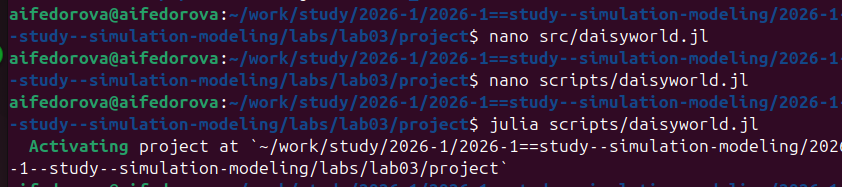
\includegraphics[keepaspectratio]{image/2.png}}

\section{Генерация
анимации}\label{ux433ux435ux43dux435ux440ux430ux446ux438ux44f-ux430ux43dux438ux43cux430ux446ux438ux438}

\pandocbounded{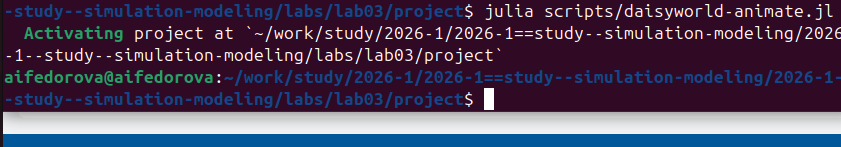
\includegraphics[keepaspectratio]{image/3.png}}

\section{Построение графика
численности}\label{ux43fux43eux441ux442ux440ux43eux435ux43dux438ux435-ux433ux440ux430ux444ux438ux43aux430-ux447ux438ux441ux43bux435ux43dux43dux43eux441ux442ux438}

\pandocbounded{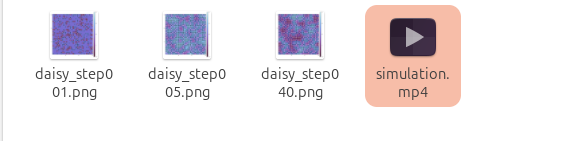
\includegraphics[keepaspectratio]{image/4.png}}

\pandocbounded{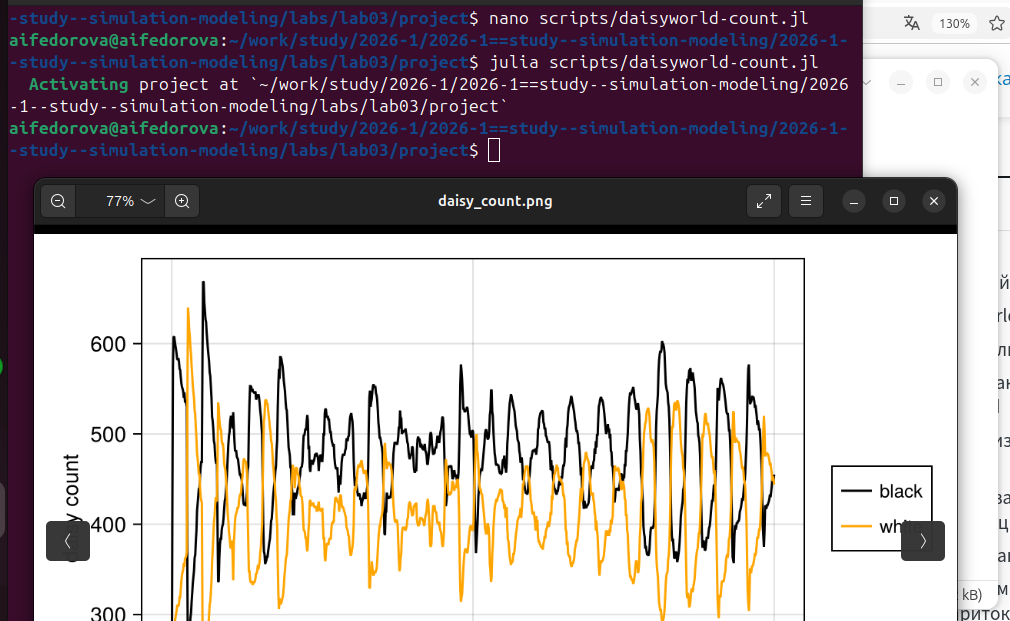
\includegraphics[keepaspectratio]{image/5.png}}

\section{Построение комплексного
графика}\label{ux43fux43eux441ux442ux440ux43eux435ux43dux438ux435-ux43aux43eux43cux43fux43bux435ux43aux441ux43dux43eux433ux43e-ux433ux440ux430ux444ux438ux43aux430}

\pandocbounded{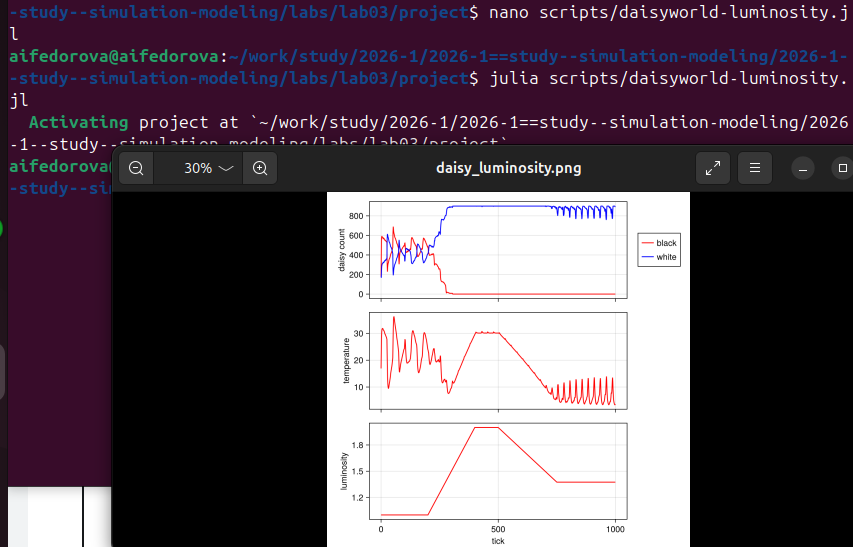
\includegraphics[keepaspectratio]{image/6.png}}

\pandocbounded{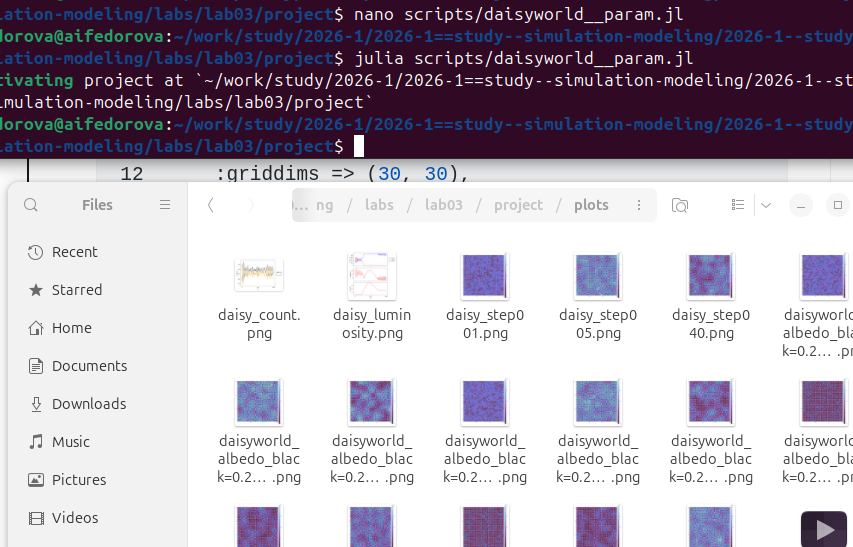
\includegraphics[keepaspectratio]{image/7.png}}

\section{Параметрические
эксперименты}\label{ux43fux430ux440ux430ux43cux435ux442ux440ux438ux447ux435ux441ux43aux438ux435-ux44dux43aux441ux43fux435ux440ux438ux43cux435ux43dux442ux44b-1}

\pandocbounded{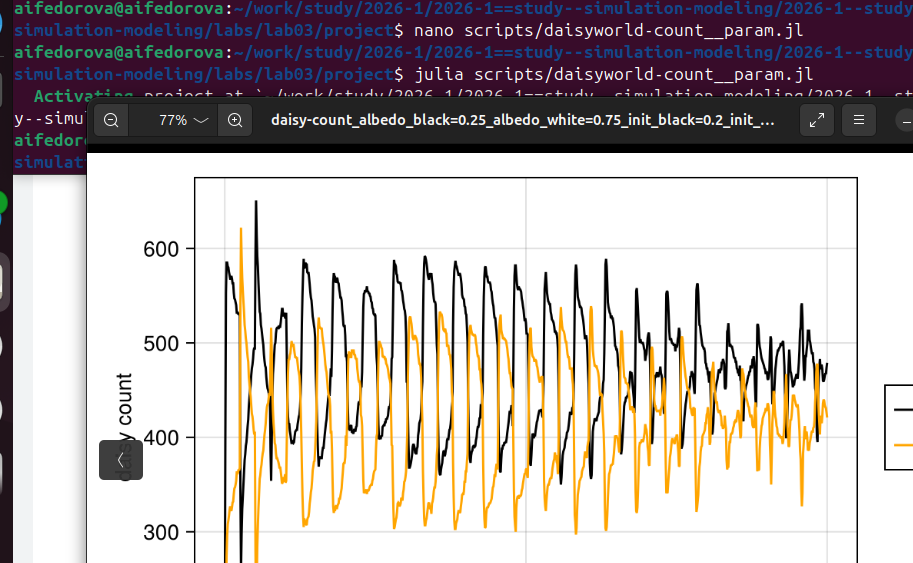
\includegraphics[keepaspectratio]{image/8.png}}

\pandocbounded{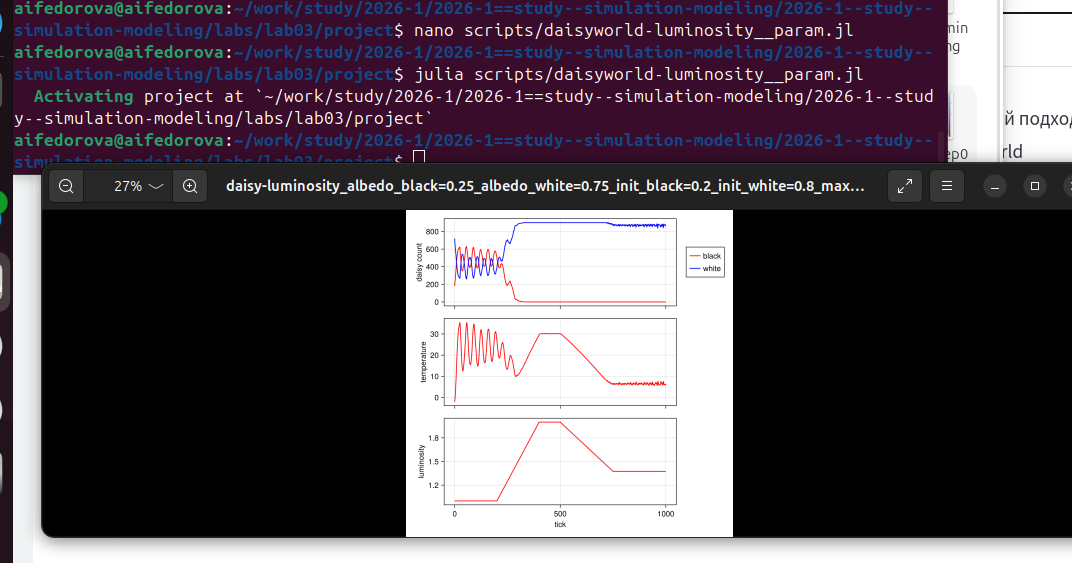
\includegraphics[keepaspectratio]{image/9.png}}

\chapter{Выводы}\label{ux432ux44bux432ux43eux434ux44b}

В ходе лабораторной работы:

\begin{itemize}
\tightlist
\item
  реализована агентная модель Daisyworld
\item
  выполнена визуализация и анализ
\item
  исследовано влияние параметров
\item
  подтверждён эффект саморегуляции
\end{itemize}

\chapter{Список
литературы}\label{ux441ux43fux438ux441ux43eux43a-ux43bux438ux442ux435ux440ux430ux442ux443ux440ux44b}

\begin{enumerate}
\def\labelenumi{\arabic{enumi}.}
\tightlist
\item
  Watson A.J., Lovelock J.E.
\item
  Datseris G. Agents.jl
\item
  Wood A.J. Daisyworld review
\end{enumerate}


\printbibliography



\end{document}
